\documentclass{article}
\usepackage[utf8]{inputenc}

% Page setup
\usepackage[a4paper,landscape,margin=2cm]{geometry}
\usepackage{amsmath}

% Typography
\usepackage[scaled]{helvet}
\let\familydefault\sfdefault

\usepackage[usenames,svgnames]{xcolor}
\usepackage{tikz,pgfplots}
\usetikzlibrary{positioning,arrows,intersections}

\definecolor{colorstore} {RGB}{199,212,104}
\definecolor{colorlayer} {RGB}{79 ,142,209}
\definecolor{colorrules} {RGB}{143,232,186}

\definecolor{colordelta}    {RGB}{199,212,104}
\definecolor{colorsnapshot} {RGB}{79 ,142,209}
\definecolor{colordict}     {RGB}{143,232,186}
\definecolor{colorhdt}      {RGB}{49 ,167,226}
\definecolor{colortext}     {RGB}{29 ,29 ,27 }

\begin{document}
\pagestyle{empty}
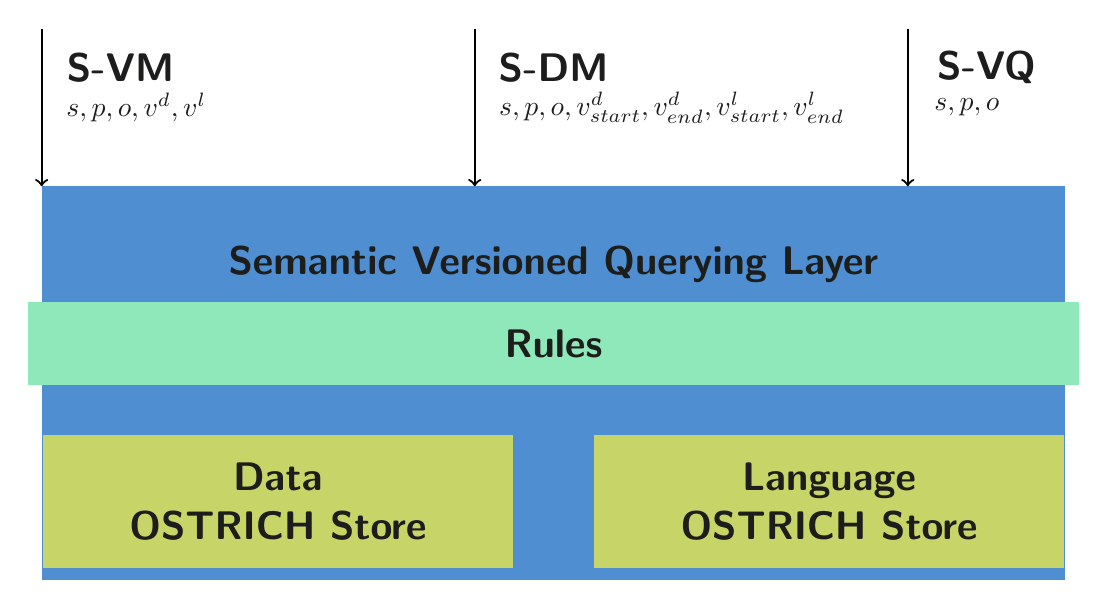
\begin{tikzpicture}[
    node distance = 2em, auto,
    font={\Large\itshape},
    base/.style={text=colortext,font={\Large\bfseries},inner sep=10pt,align=center,rectangle},
    txt/.style={text=colortext,font={\Large\bfseries},align=center},
    treenode/.style={base,thick,draw=colortext,text width=2em},
    relation/.style={text width=13em},
]

    % Layer
    \fill[colorlayer] (-3, 3) rectangle (10, -2);
    \node[base,fill=colorlayer,text width=30em] at (3.5, 2) (layer) {Semantic Versioned Querying Layer};

    % Stores
    \node[base,fill=colorrules,text width=36em] at ( 3.5, 1) (rules) {Rules};
    \node[base,fill=colorstore,text width=15em] at ( 0, -1) (data) {Data\\OSTRICH Store};
    \node[base,fill=colorstore,text width=15em] at ( 7, -1) (language)   {Language\\OSTRICH Store};
    
    % Queries
    \draw[->,thick](-3,5) to (-3,3);
    \draw[->,thick](2.5,5) to (2.5,3);
    \draw[->,thick](8,5) to (8,3);
    \node[txt] at (-2,4.5) {S-VM};
    \node[txt,font={}] at (-1.8,4) {$s,p,o,v^d,v^l$};
    \node[txt] at (3.5,4.5) {S-DM};
    \node[txt,font={}] at (5,4) {$s,p,o,v^d_{start},v^d_{end},v^l_{start},v^l_{end}$};
    \node[txt] at (9,4.5) {S-VQ};
    \node[txt,font={}] at (8.75,4) {$s,p,o$};

\end{tikzpicture}
\end{document}
